\newpage
\clearpage
\onecolumn
\section{Example Appendix}
\label{sec:appendix}

% \subsection{Prompt Templates}
% \begin{table}[h]
\centering
\small
\begin{tabular}{|p{0.92\linewidth}|}
\hline
\texttt{\textbf{\{StructEval Question\}}} \\
\texttt{} \\
\texttt{IMPORTANT: Only output the required output format. You must start the format/code with <|BEGIN\_CODE|> and end the format/code with <|END\_CODE|>. No other text output (explanation, comments, etc.) are allowed.} \\
\texttt{Do not use markdown code fences.} \\
\hline
\end{tabular}
\caption{Prompt template used for LLM inference before the evaluation}
\label{tab:prompt_template}
\end{table}


\subsection{Task Distributions}
% Please add the following required packages to your document preamble:
% \usepackage{multirow}
\begin{table}[!ht]
\centering
\resizebox{0.45\textwidth}{!}{
\begin{tabular}{ccc}
\toprule
\textbf{Subset} & \textbf{Tasks} & \textbf{\# Examples} \\
\midrule
\multicolumn{3}{c}{\textbf{Generation}} \\
\midrule
\multirow{5}{*}{StructEval-T} & Text $\rightarrow$ JSON & 50 \\
 & Text $\rightarrow$ CSV & 50 \\
 & Text $\rightarrow$ TOML & 50 \\
 & Text $\rightarrow$ XML & 50 \\
 & Text $\rightarrow$ YAML & 50 \\
\noalign{\vskip 2pt}
\midrule
\noalign{\vskip 2pt}
\multirow{13}{*}{StructEval-V} & Text $\rightarrow$ Angular & 50 \\
 & Text $\rightarrow$ Canvas & 50 \\
 & Text $\rightarrow$ HTML & 50 \\
 & Text $\rightarrow$ LaTeX & 50 \\
 & Text $\rightarrow$ Markdown & 50 \\
 & Text $\rightarrow$ Matplotlib & 50 \\
 & Text $\rightarrow$ Mermaid & 50 \\
 & Text $\rightarrow$ React & 50 \\
 & Text $\rightarrow$ SVG & 50 \\
 & Text $\rightarrow$ TikZ & 50 \\
 & Text $\rightarrow$ Typst & 50 \\
 & Text $\rightarrow$ Vega & 50 \\
 & Text $\rightarrow$ Vue & 50 \\
\midrule
\multicolumn{3}{c}{\textbf{Conversion}} \\
\midrule
\multirow{14}{*}{StructEval-T} & CSV $\rightarrow$ JSON & 50 \\
 & JSON $\rightarrow$ CSV & 50 \\
 & XML $\rightarrow$ JSON & 50 \\
 & JSON $\rightarrow$ XML & 50 \\
 & YAML $\rightarrow$ JSON & 50 \\
 & JSON $\rightarrow$ YAML & 50 \\
 & XML $\rightarrow$ CSV & 50 \\
 & CSV $\rightarrow$ XML & 50 \\
 & XML $\rightarrow$ YAML & 50 \\
 & YAML $\rightarrow$ XML & 50 \\
 & YAML $\rightarrow$ CSV & 50 \\
 & TOML $\rightarrow$ JSON & 50 \\
 & CSV $\rightarrow$ YAML & 50 \\
 & TOML $\rightarrow$ YAML & 50 \\
\noalign{\vskip 2pt}
\midrule
\noalign{\vskip 2pt}
\multirow{12}{*}{StructEval-V} & Matplotlib $\rightarrow$ TikZ & 100 \\
 & Markdown $\rightarrow$ HTML & 50 \\
 & HTML $\rightarrow$ React & 45 \\
 & React $\rightarrow$ HTML & 45 \\
 & Vue $\rightarrow$ HTML & 40 \\
 & HTML $\rightarrow$ Vue & 40 \\
 & Markdown $\rightarrow$ React & 30 \\
 & HTML $\rightarrow$ Angular & 30 \\
 & Markdown $\rightarrow$ Vue & 25 \\
 & Vue $\rightarrow$ React & 15 \\
 & Markdown $\rightarrow$ Angular & 10 \\
 & React $\rightarrow$ Angular & 5 \\
 \bottomrule
\end{tabular}}
\caption{Statistics of number examples for each task in all the 4 subsets of \structeval.}
\label{tab:task_dist}
\end{table}

\newpage
\clearpage
\subsection{Subtask Performance}
\label{appendix:subtask_perf}
\begin{table*}[ht]
\centering
\small
\label{tab:structeval_t_gen}
\resizebox{0.9\linewidth}{!}{
\begin{tabular*}{\textwidth}{@{\extracolsep{\fill}}l*{5}{S[table-format=3.2]}S[table-format=3.2]}
\toprule
\textbf{Model} &
\rotatebox{60}{T$\!\to\!$JSON} &
\rotatebox{60}{T$\!\to\!$CSV}  &
\rotatebox{60}{T$\!\to\!$TOML} &
\rotatebox{60}{T$\!\to\!$XML}  &
\rotatebox{60}{T$\!\to\!$YAML} &
\textbf{Avg.} \\
\midrule
Llama-3.1-8B-Instruct     & 78.82 & 81.68 &  6.76 & 59.38 & 74.44 & 60.22 \\
Meta-Llama-3-8B-Instruct  & 69.08 & 45.04 &  7.94 & 45.30 & 78.54 & 49.18 \\
Phi-3-mini-128k-Instruct  & 68.84 & \textbf{93.50} &  0.00 & 37.68 & 36.92 & 47.39 \\
Phi-4-mini-Instruct       & 51.50 & 82.56 & 16.12 & 40.20 & 66.54 & 51.38 \\
Qwen-2.5-7B-Instruct      & 84.40 & 90.62 & 13.22 & 61.30 & 46.52 & 59.21 \\
Qwen-3-4B               & 90.96 & 76.44 &  7.44 & 71.16 & 78.74 & 64.95 \\
Gemini-1.5-pro          & 94.06 & \textbf{100.00} & 75.38 & 73.32 & \textbf{97.58} & 88.07 \\
Gemini-2.0-flash        & 48.88 & 98.40 & 78.78 & 44.60 & 91.44 & 72.42 \\
GPT-4.1-mini            & \textbf{99.26} & 99.92 & \textbf{91.34} & \textbf{77.06} & 95.26 & \textbf{92.57} \\
GPT-4o                  & \textbf{99.36} & \textbf{100.00} & 90.22 & 70.32 & \textbf{97.68} & 91.52 \\
GPT-4o-mini             & 97.88 & 99.90 & 29.56 & 75.10 & 96.84 & 79.86 \\
o1-mini                 & 92.56 & 99.24 & 89.40 & 71.12 & 88.28 & 88.12 \\
\bottomrule
\end{tabular*}}
\caption{StructEval-T Generation Scores}
\end{table*}

\begin{table*}[ht]
\centering
\scriptsize
\label{tab:structeval_v_gen_a}
\begin{tabular*}{\textwidth}{@{\extracolsep{\fill}}l*{7}{S[table-format=3.2]}}
\toprule
\textbf{Model} &
\rotatebox{60}{T$\!\to\!$Ang.} & \rotatebox{60}{T$\!\to\!$\LaTeX} &
\rotatebox{60}{T$\!\to\!$MD}   & \rotatebox{60}{T$\!\to\!$MPL}  &
\rotatebox{60}{T$\!\to\!$React}& \rotatebox{60}{T$\!\to\!$SVG}  &
\rotatebox{60}{T$\!\to\!$TikZ}\\
\midrule
Llama-3.1-8B-Instruct   & 61.22 & 78.04 & 87.34 & 80.52 & 64.30 & 44.18 & 46.92 \\
Meta-Llama-3-8B-Instruct& 48.92 & 68.40 & 72.06 & 56.54 & 55.24 & 40.16 & 28.04 \\
Phi-3-mini-128k-Instruct& 48.28 & 63.88 & 64.16 & 59.38 & 44.12 & 35.78 & 32.44 \\
Phi-4-mini-Instruct      & 62.60 & 72.92 & 88.90 & 71.30 & 58.46 & 39.72 & 35.28 \\
Qwen-2.5-7B-Instruct     & 63.08 & 66.68 & 81.02 & 74.70 & 65.48 & 47.30 & 48.88 \\
Qwen-3-4B              & 48.80 & 72.60 & \textbf{92.80} & 89.54 & \textbf{77.06} & 53.44 & 55.38 \\
Gemini-1.5-pro         & \textbf{90.62} & 76.94 & 94.00 & 84.96 & 33.68 & 54.72 & 69.44 \\
Gemini-2.0-flash       & 44.28 & 75.26 & 92.06 & 75.34 & 46.64 & \textbf{56.72} & 61.24 \\
GPT-4.1-mini           & 84.52 & 76.20 & 91.80 & \textbf{96.34} & 69.58 & 58.74 & 69.74 \\
GPT-4o                 & 87.42 & 75.18 & 93.02 & 95.76 & 74.66 & 56.78 & 62.32 \\
GPT-4o-mini            & 86.72 & \textbf{78.44} & 94.36 & 95.36 & 75.46 & 53.98 & 60.76 \\
o1-mini                & 89.30 & 49.24 & 92.08 & 96.06 & 71.98 & 58.12 & \textbf{71.86} \\
\bottomrule
\end{tabular*}
\caption{StructEval-V Generation Scores (Part 1)}
\end{table*}

\begin{table*}[ht]
\centering
\scriptsize
\begin{tabular*}{\textwidth}{@{\extracolsep{\fill}}l*{6}{S[table-format=3.2]}S[table-format=3.2]}
\toprule
\textbf{Model} &
\rotatebox{60}{T$\!\to\!$HTML} &
\rotatebox{60}{T$\!\to\!$Mermaid} &
\rotatebox{60}{T$\!\to\!$Typst} &
\rotatebox{60}{T$\!\to\!$Vega}  &
\rotatebox{60}{T$\!\to\!$Vue}   &
\rotatebox{60}{T$\!\to\!$Canvas} &
\textbf{Avg.}\\
\midrule
Llama-3.1-8B-Instruct   & 95.96 &  9.02 & 23.38 & 28.36 & 57.90 & 30.56 & 54.44 \\
Meta-Llama-3-8B-Instruct& 72.52 &  6.04 & 29.46 & 30.74 & \textbf{66.50} & 31.28 & 46.61 \\
Phi-3-mini-128k-Instruct& 92.10 & 11.12 & 22.90 & 35.56 & 39.84 & 32.50 & 44.77 \\
Phi-4-mini-Instruct      & 97.24 &  9.30 & 42.22 & 34.72 & 29.48 & 28.90 & 51.62 \\
Qwen-2.5-7B-Instruct     & 92.92 &  6.16 & 33.44 & 30.56 & 37.90 & 44.52 & 53.28 \\
Qwen-3-4B              & 98.80 & 13.62 &  9.92 & 45.28 & 29.42 & \textbf{54.28} & 57.00 \\
Gemini-1.5-pro         & \textbf{99.30} & 15.94 & 11.60 & \textbf{65.18} & 29.66 & 29.36 & 58.11 \\
Gemini-2.0-flash       & 99.26 &  9.66 & \textbf{45.28} & 29.74 & 32.46 & 29.16 & 53.62 \\
GPT-4.1-mini           & 99.30 & \textbf{43.46} &  9.96 & 48.28 & 38.44 & 49.60 & 64.30 \\
GPT-4o                 & 99.22 & 36.00 & 23.94 & \textbf{72.20} & 40.04 & 33.54 & \textbf{65.39} \\
GPT-4o-mini            & 99.02 & 30.50 &  9.96 & 41.28 & 33.66 & 30.50 & 60.77 \\
o1-mini                & \textbf{99.44} & 27.76 &  9.98 & 65.68 & \textbf{40.76} & 33.52 & 61.98 \\
\bottomrule
\end{tabular*}
\caption{StructEval-V Generation Scores (Part 2)}
\label{tab:structeval_v_gen_b}
\end{table*}

% =====================================================================

\begin{table*}[ht]
\centering
\scriptsize
\resizebox{0.95\linewidth}{!}{
\begin{tabular*}{\textwidth}{@{\extracolsep{\fill}}l*{7}{S[table-format=3.2]}}
\toprule
\textbf{Model} &
\rotatebox{60}{C$\!\to\!$JSON} &
\rotatebox{60}{J$\!\to\!$CSV} &
\rotatebox{60}{X$\!\to\!$JSON} &
\rotatebox{60}{J$\!\to\!$XML} &
\rotatebox{60}{Y$\!\to\!$JSON} &
\rotatebox{60}{J$\!\to\!$YAML} &
\rotatebox{60}{X$\!\to\!$CSV}\\
\midrule
Llama-3.1-8B-Instruct& 34.14 & 95.96 & 68.62 & 56.02 & 94.00 & 92.52 & 98.98 \\
Meta-Llama-3-8B-Instruct& 31.40 & 48.00 & 69.24 & 55.40 & 90.00 & 74.00 & 48.26 \\
Phi-3-mini-128k-Instruct& 24.88 & 87.28 &  8.00 & 12.40 & 23.20 & 32.80 & 33.92 \\
Phi-4-mini-Instruct& 45.42 & 97.62 & 89.56 & 61.90 & \textbf{100.00} & \textbf{100.00} & 90.70 \\
Qwen-2.5-7B-Instruct& 31.36 & 95.74 & 33.14 & 31.04 & 50.00 & 95.24 & 77.72 \\
Qwen-3-4B& 55.28 & \textbf{100.00} & \textbf{92.84} & 65.98 & \textbf{100.00} & 98.00 & \textbf{99.78} \\
Gemini-1.5-pro& 48.14 & \textbf{100.00} & 40.14 & 67.14 & 98.00 & \textbf{100.00} & \textbf{99.78} \\
Gemini-2.0-flash& 25.72 & \textbf{100.00} & 32.60 & \textbf{69.76} & \textbf{100.00} & \textbf{100.00} & \textbf{99.78} \\
GPT-4.1-mini& \textbf{55.52} & \textbf{100.00} & 38.68 & \textbf{69.76} & \textbf{100.00} & \textbf{100.00} & \textbf{99.78} \\
GPT-4o& 38.56 & 99.74 & 66.46 & \textbf{69.76} & \textbf{100.00} & \textbf{100.00} & \textbf{99.78} \\
GPT-4o-mini& \textbf{58.52} & \textbf{100.00} & 73.26 & 65.98 & 98.00 & \textbf{100.00} & 98.22 \\
o1-mini& 58.46 & \textbf{100.00} & 82.70 & 68.60 & \textbf{100.00} & \textbf{100.00} & \textbf{99.78} \\
\bottomrule
\end{tabular*}}
\caption{StructEval-T Conversion Scores (Part 1)}
\label{tab:structeval_t_conv_a}
\end{table*}

\begin{table*}[ht]
\centering
\scriptsize
\resizebox{0.95\linewidth}{!}{
\begin{tabular*}{\textwidth}{@{\extracolsep{\fill}}l*{8}{S[table-format=3.2]}}
\toprule
\textbf{Model} &
\rotatebox{60}{C$\!\to\!$XML} &
\rotatebox{60}{X$\!\to\!$YAML} &
\rotatebox{60}{Y$\!\to\!$XML} &
\rotatebox{60}{Y$\!\to\!$CSV} &
\rotatebox{60}{Toml$\!\to\!$JSON} &
\rotatebox{60}{C$\!\to\!$YAML} &
\rotatebox{60}{Toml$\!\to\!$YAML} &
\textbf{Avg.}\\
\midrule
Llama-3.1-8B-Instruct& 20.20 & 86.96 & 39.90 & 88.32 & 86.90 & 49.54 & 85.62 & 71.26 \\
Meta-Llama-3-8B-Instruct& 17.28 & 54.48 & 38.12 & 61.90 & 63.38 & 36.50 & 63.18 & 53.65 \\
Phi-3-mini-128k-Instruct&  9.50 & 20.56 & 22.42 & \textbf{87.58} &  8.80 & 19.10 & 26.46 & 29.78 \\
Phi-4-mini-Instruct& 21.72 & 60.00 & 48.28 & 84.14 & 86.02 & 66.22 & 61.84 & 72.39 \\
Qwen-2.5-7B-Instruct& 18.12 & 81.62 & 24.16 & \textbf{97.62} & 78.22 & 70.86 & 85.68 & 62.18 \\
Qwen-3-4B& 24.82 & \textbf{94.10} & 48.68 & \textbf{98.94} & 96.92 & 65.08 & \textbf{95.36} & 81.13 \\
Gemini-1.5-pro& 27.14 & 42.96 & 47.56 & \textbf{100.00} & 99.76 & 71.40 & 97.36 & 74.24 \\
Gemini-2.0-flash& 17.74 & 59.02 & 46.36 & \textbf{100.00} & 99.26 & 63.18 & 97.36 & 72.20 \\
GPT-4.1-mini& \textbf{29.36} & 59.18 & 48.36 & \textbf{100.00} & \textbf{100.00} & 60.82 & 97.36 & 75.63 \\
GPT-4o& 27.40 & 44.28 & 48.76 & \textbf{100.00} & \textbf{100.00} & 43.20 & 97.36 & 73.95 \\
GPT-4o-mini& 29.62 & 40.20 & \textbf{48.76} & 98.10 & \textbf{100.00} & 50.00 & 97.36 & 75.57 \\
o1-mini& 29.26 & 88.62 & 48.36 & \textbf{100.00} & \textbf{100.00} & \textbf{72.40} & 97.36 & 81.82 \\
\bottomrule
\end{tabular*}}
\caption{StructEval-T Conversion Scores (Part 2)}
\label{tab:structeval_t_conv_b}
\end{table*}

\begin{table*}[ht]
\centering
\scriptsize
\resizebox{0.95\linewidth}{!}{
\begin{tabular*}{\textwidth}{@{\extracolsep{\fill}}l*{6}{S[table-format=3.2]}}
\toprule
\textbf{Model} &
\rotatebox{60}{R$\!\to\!$HTML} &
\rotatebox{60}{V$\!\to\!$HTML} &
\rotatebox{60}{MD$\!\to\!$React} &
\rotatebox{60}{HTML$\!\to\!$Ang.} &
\rotatebox{60}{MD$\!\to\!$Vue} &
\rotatebox{60}{MPL$\!\to\!$TikZ}\\
\midrule
Llama-3.1-8B-Instruct& 88.36 & 84.65 & 43.23 & 60.90 & 36.36 & 16.26 \\
Meta-Llama-3-8B-Instruct& 86.82 & 85.23 & 33.73 & 52.83 & 29.52 &  8.29 \\
Phi-3-mini-128k-Instruct& 70.73 & 73.85 & 30.80 & 32.77 & 27.32 & 17.15 \\
Phi-4-mini-Instruct& 92.27 & 81.82 & 28.50 & 33.47 & 33.88 & 15.70 \\
Qwen-2.5-7B-Instruct& 89.29 & 79.53 & 34.70 & 68.67 & 33.80 & 26.32 \\
Qwen-3-4B& \textbf{95.53} & 89.65 & 54.23 & 55.10 & 34.64 & 25.64 \\
Gemini-1.5-pro& 95.24 & \textbf{91.27} & 34.83 & \textbf{86.43} & 30.96 & 38.82 \\
Gemini-2.0-flash& 93.02 & 88.67 & 32.37 & 29.30 & 32.00 & 17.46 \\
GPT-4.1-mini& 95.22 & 90.12 & 52.87 & 81.97 & 31.96 & 36.80 \\
GPT-4o& 95.36 & 90.55 & 74.20 & 87.17 & \textbf{37.56} & 39.69 \\
GPT-4o-mini& 95.07 & \textbf{91.58} & \textbf{80.40} & \textbf{87.73} & 31.96 & \textbf{42.47} \\
o1-mini& 95.09 & 89.65 & 58.37 & 87.90 & 36.80 & 40.60 \\
\bottomrule
\end{tabular*}}
\caption{StructEval-V Conversion Scores (Part 1)}
\label{tab:structeval_v_conv_a}
\end{table*}

\begin{table*}[ht]
\centering
\scriptsize
\resizebox{0.95\linewidth}{!}{
\begin{tabular*}{\textwidth}{@{\extracolsep{\fill}}l*{7}{S[table-format=3.2]}}
\toprule
\textbf{Model} &
\rotatebox{60}{MD$\!\to\!$HTML} &
\rotatebox{60}{HTML$\!\to\!$React} &
\rotatebox{60}{HTML$\!\to\!$Vue} &
\rotatebox{60}{V$\!\to\!$React} &
\rotatebox{60}{MD$\!\to\!$Ang.} &
\rotatebox{60}{R$\!\to\!$Ang.} &
\textbf{Avg.}\\
\midrule
Llama-3.1-8B-Instruct& 88.28 & 55.02 & 72.93 & 75.73 & 26.90 & 85.20 & 61.15 \\
Meta-Llama-3-8B-Instruct& 84.52 & 73.91 & 75.28 & 62.73 & 33.10 & 57.00 & 56.91 \\
Phi-3-mini-128k-Instruct& 65.60 & 42.16 & 34.65 & 33.00 & 25.10 & 41.60 & 41.23 \\
Phi-4-mini-Instruct& 92.44 & 57.11 & 41.05 & 55.87 & 26.50 & 71.20 & 52.48 \\
Qwen-2.5-7B-Instruct& 85.16 & 69.20 & 80.02 & 50.87 & 35.00 & 84.60 & 61.43 \\
Qwen-3-4B& 90.20 & 65.31 & \textbf{83.05} & 68.13 & 34.50 & 85.00 & 65.08 \\
Gemini-1.5-pro& 95.28 & 40.62 & \textbf{86.65} & 64.00 & \textbf{49.80} & 85.20 & 66.59 \\
Gemini-2.0-flash& \textbf{96.60} & 41.04 & 67.77 & 68.00 & 28.20 & 29.20 & 51.97 \\
GPT-4.1-mini& 96.40 & \textbf{88.09} & 46.28 & \textbf{86.47} & 49.10 & 85.20 & 70.04 \\
GPT-4o& 95.32 & 88.31 & 62.55 & 78.93 & 48.20 & 80.60 & 73.20 \\
GPT-4o-mini& 93.14 & \textbf{88.42} & 79.75 & \textbf{81.20} & 49.20 & \textbf{97.60} & \textbf{76.54} \\
o1-mini& 94.48 & 72.18 & 77.77 & 65.60 & 41.20 & 85.20 & 70.40 \\
\bottomrule
\end{tabular*}}
\caption{StructEval-V Conversion Scores (Part 2)}
\label{tab:structeval_v_conv_b}
\caption*{\footnotesize* T - Text, C – CSV, J – JSON, X – XML, Y – YAML, Ang. – Angular, MD – Markdown, MPL – Matplotlib, R – React, V – Vue.}
\end{table*}


\newpage
\clearpage

\subsection{Examples of rendered image}
\label{appendix:rendered_images}
\begin{figure*}[!h]
  \centering
  \captionsetup[subfigure]{justification=centering}

  \newlength{\imgH}\setlength{\imgH}{3.6cm}  % uniform height

  % ---------- first row ----------
  \begin{subfigure}{0.32\textwidth}
    \centering
    \fcolorbox{imgborder}{white}{%
      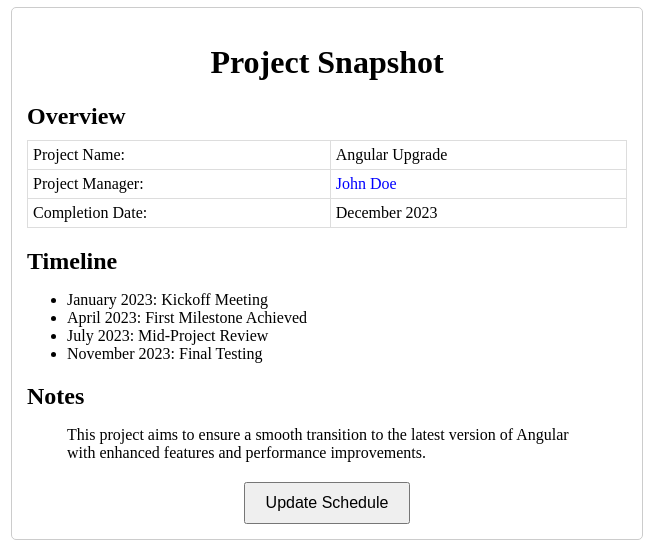
\includegraphics[height=\imgH,keepaspectratio]{images/000107.png}}
    \caption{Angular}
  \end{subfigure}\hfill
  \begin{subfigure}{0.32\textwidth}
    \centering
    \fcolorbox{imgborder}{white}{%
      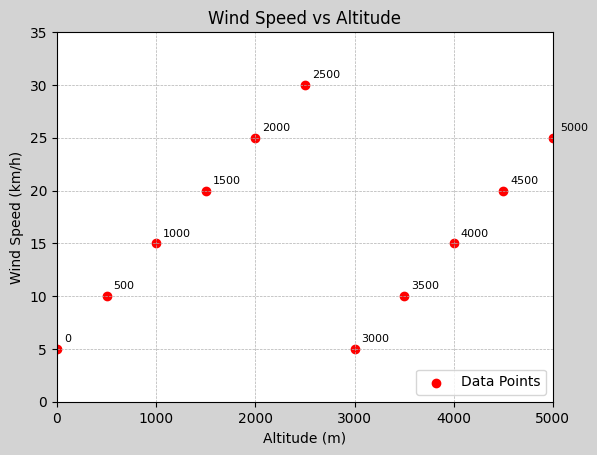
\includegraphics[height=\imgH,keepaspectratio]{images/000829.png}}
    \caption{Matplotlib}
  \end{subfigure}\hfill
  \begin{subfigure}{0.32\textwidth}
    \centering
    \fcolorbox{imgborder}{white}{%
      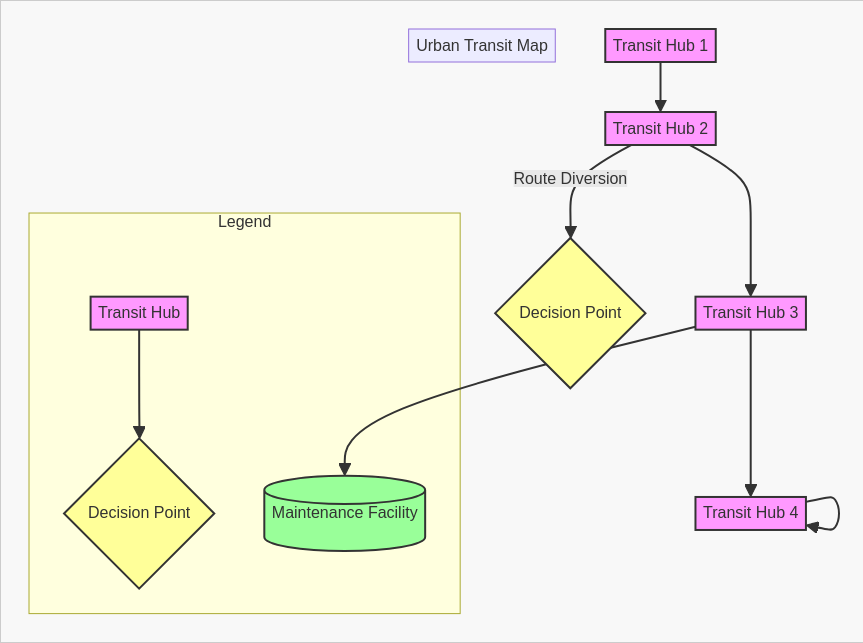
\includegraphics[height=\imgH,keepaspectratio]{images/000936.png}}
    \caption{Mermaid}
  \end{subfigure}

  \vspace{0.6em}

  % ---------- second row ----------
  \begin{subfigure}{0.32\textwidth}
    \centering
    \fcolorbox{imgborder}{white}{%
      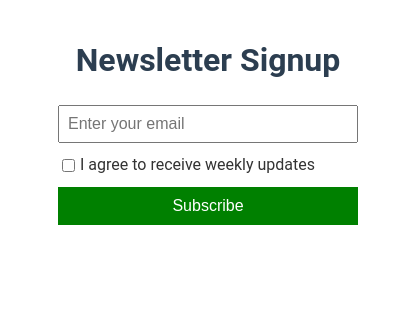
\includegraphics[height=\imgH,keepaspectratio]{images/001126.png}}
    \caption{React}
  \end{subfigure}\hfill
  \begin{subfigure}{0.32\textwidth}
    \centering
    \fcolorbox{imgborder}{white}{%
      
\includegraphics[height=\imgH,keepaspectratio]{images/001210.png}}
    \caption{SVG}
  \end{subfigure}\hfill
  \begin{subfigure}{0.32\textwidth}
    \centering
    \fcolorbox{imgborder}{white}{%
      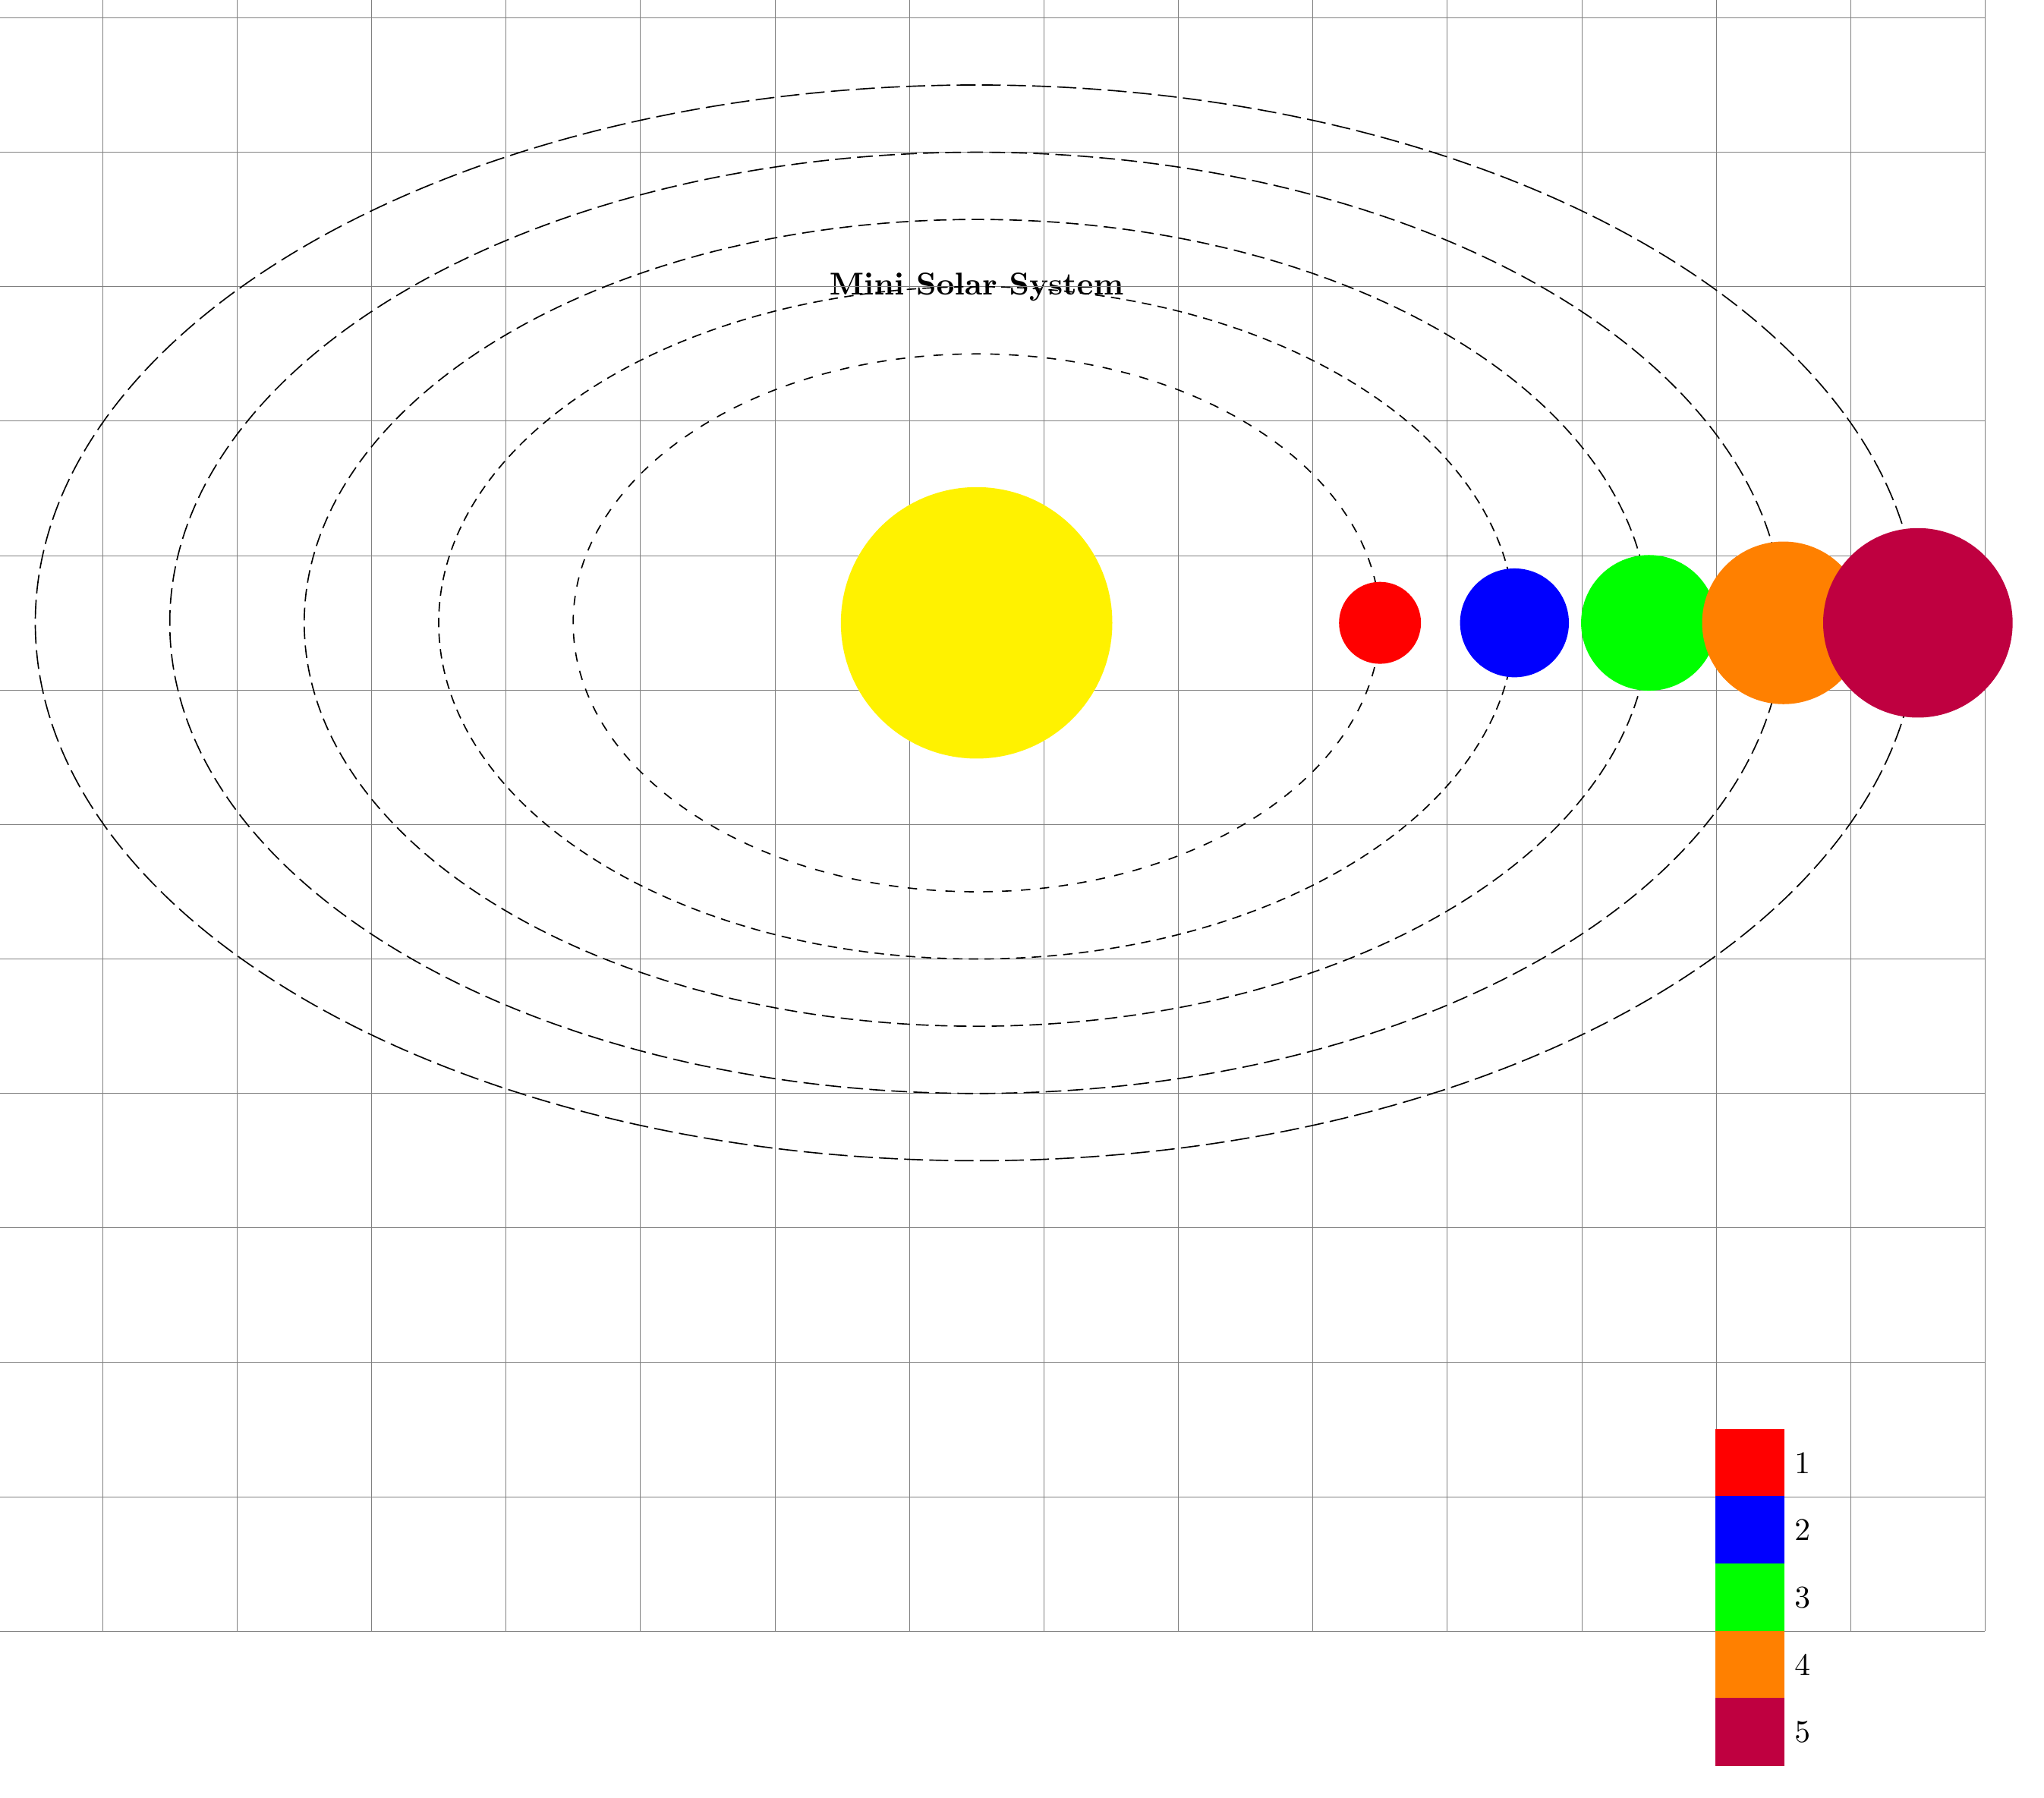
\includegraphics[height=\imgH,keepaspectratio]{images/001312.png}}
    \caption{TikZ}
  \end{subfigure}

  \vspace{0.6em}

  % ---------- third row ----------
  \begin{subfigure}{0.32\textwidth}
    \centering
    \fcolorbox{imgborder}{white}{%
      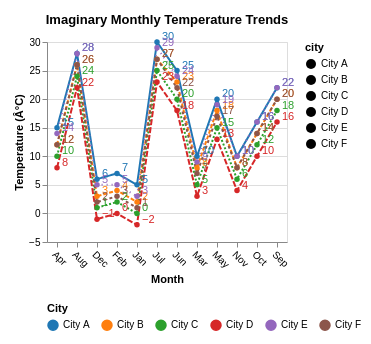
\includegraphics[height=\imgH,keepaspectratio]{images/001509.png}}
    \caption{Vega}
  \end{subfigure}

  \caption{Example images rendered in \structeval tasks.}
  \label{fig:rendered_images}
\end{figure*}

\newpage
\clearpage

\subsection{Task Generation Prompt}
\label{appendix:task_prompt}

\begin{figure}[!th]

  \begin{tcolorbox}[
    colback=white,
    colframe=gray!70,
    title={\small\bfseries Sample Prompt},
    colbacktitle=gray!10,
    coltitle=black,
    fontupper=\small,
    enhanced,
    left=2mm,
    right=2mm,
    boxrule=0.4pt,
    arc=1mm
  ]
You are a prompt-design assistant building benchmark items for conversion tasks.

\textbf{Input Format:} \{input\_type\} \\
\textbf{Output Format:} \{output\_type\}

\textbf{Your task:} Think silently through the checklist and then output a single JSON object with:
\begin{itemize}
  \item \texttt{"raw\_output\_metric"}: dot-paths for the expected keys/attributes in the \{output\_type\} structure
  \item \texttt{"query"}: A generated input format \{input\_type\} code inside \texttt{<code>...</code>} tags.
\end{itemize}

\textbf{Assumed Mapping Rule (state it implicitly in the paths):}
\begin{itemize}
  \item \textbf{No XML attributes} unless absolutely necessary. \\
        If an attribute is required, map it to a key prefixed with \texttt{"@"}, and include that in dot-paths.
\end{itemize}

\hrulefill \\
\textbf{CHECKLIST (INTERNAL – DO NOT OUTPUT)}
\begin{enumerate}
  \item Pick a super creative and random domain.
  \item Generate \{input\_type\} code with:
    \begin{itemize}
      \item At least two levels of nesting
      \item At least one list inside an object/element
    \end{itemize}
  \item Avoid XML attributes where possible; prefer child elements.
  \item Wrap the code in \texttt{<code>...</code>} tags.
  \item Dot-path rules:
    \begin{itemize}
      \item JSON / YAML / TOML: \texttt{parent.child}, \texttt{list[0].child}
      \item XML: \texttt{element.child} or \texttt{element.@attr} (only if used)
      \item CSV: \texttt{csv::Header} (not used here)
    \end{itemize}
\end{enumerate}

\hrulefill \\
\textbf{OUTPUT FORMAT}
\begin{verbatim}
{
  "raw_output_metric": ["<dot_path1>",
                        "<dot_path2>", ...],
  "query": "<code>...</code>"
}
\end{verbatim}

  \end{tcolorbox}
  \caption{Example task generation prompt}
  \label{fig:sample_task_prompt}
\end{figure}